%%%%%%%%%%%%%%%%%%%%%%%%%%%%%%%%%%%%%%%%%
% Thin Sectioned Essay
% LaTeX Template
% Version 1.0 (3/8/13)
%
% This template has been downloaded from:
% http://www.LaTeXTemplates.com
%
% Original Author:
% Nicolas Diaz (nsdiaz@uc.cl) with extensive modifications by:
% Vel (vel@latextemplates.com)
%
% License:
% CC BY-NC-SA 3.0 (http://creativecommons.org/licenses/by-nc-sa/3.0/)
%
%%%%%%%%%%%%%%%%%%%%%%%%%%%%%%%%%%%%%%%%%

%----------------------------------------------------------------------------------------
%	PACKAGES AND OTHER DOCUMENT CONFIGURATIONS
%----------------------------------------------------------------------------------------

\documentclass[a4paper, 11pt]{article} % Font size (can be 10pt, 11pt or 12pt) and paper size (remove a4paper for US letter paper)

\usepackage[protrusion=true,expansion=true]{microtype} % Better typography
\usepackage{graphicx} % Required for including pictures
\usepackage{wrapfig} % Allows in-line images

\usepackage{mathpazo} % Use the Palatino font
\usepackage[T1]{fontenc} % Required for accented characters
%\usepackage[backend=bibtex,style=verbose-trad2]{biblatex}
\usepackage{hyperref}
\usepackage{longtable}
\usepackage{array}
\usepackage{multirow}
\usepackage[utf8]{inputenc}
\usepackage{subcaption}
\usepackage[font=small]{caption}
\usepackage{units}
\usepackage{relsize}
\usepackage{gensymb}
\usepackage{textcomp}

\linespread{1.05} % Change line spacing here, Palatino benefits from a slight increase by default

\makeatletter
\renewcommand{\refname}{Bibliografie}
\renewcommand{\@listI}{\itemsep=0pt} % Reduce the space between items in the itemize and enumerate environments and the bibliography

\renewcommand{\maketitle}{ % Customize the title - do not edit title and author name here, see the TITLE block below
	\begin{flushright} % Right align
		{\LARGE\@title} % Increase the font size of the title
		
		\vspace{50pt} % Some vertical space between the title and author name
		
		{\large\@author} % Author name
		\\\@date % Date
		
		\vspace{40pt} % Some vertical space between the author block and abstract
	\end{flushright}
}

%----------------------------------------------------------------------------------------
%	TITLE
%----------------------------------------------------------------------------------------

\title{\textbf{Ontwerpverslag}\\ % Title
	De implementatie van een koolstofmonoxidesensor} % Subtitle

\author{\textsc{R. Bolding} % Author
	\\{\textit{Amsterdam University of Applied Sciences\\ 
			HvA\\
			Sensor Netwerken: groep 5\\
			Studentnummer: 500757732}}} % Institution

\date{9 december, 2019} % Date

%----------------------------------------------------------------------------------------
\begin{document}
	\captionsetup[figure]{labelfont={bf},name={Fig},labelsep=period}
	\captionsetup{justification=centering}
	\renewcommand{\contentsname}{Inhoudsopgave}
	\def\textsubscript#1{\ensuremath{_{\mbox{\textscale{.6}{#1}}}}}
	\hypersetup{hidelinks=true}
	\maketitle % Print the title section
	
	%----------------------------------------------------------------------------------------
	%	ABSTRACT AND KEYWORDS
	%----------------------------------------------------------------------------------------
	
	%\renewcommand{\abstractname}{Summary} % Uncomment to change the name of the abstract to something else
	
	
	\vspace{10pt} % Some vertical space between the abstract and first section
	
	%----------------------------------------------------------------------------------------
	%	ESSAY BODY
	%-----------------------------------------------
	\newpage
	\tableofcontents
	\newpage
	\section{Specificaties sensormodule} \label{sec::specificaties}
	\begin{center}
		\begin{tabular}{ | m{5cm} | m{5cm}| } 
			\hline
			\multicolumn{2}{|c|}{Specificaties voor de implementaties van CO sensoren} \\
			\hline
			Meetbereik a: & 0 - 200 \textit{ppm} \\
			\hline
			detectie limiet:  & <2 \textit{ppm}
			\\ 
			\hline
			detectie resolutie: & 2 \textit{ppm} 
			\\ 
			\hline
			responstijd: & < 3 minuut
			\\ 
			\hline
			Voed spanning: & min: 2,7V max: 3,3V
			\\ 
			\hline
			Maximaal vermogen: & 1 mW
			\\
			\hline
			Output gevoeligheid: & 1mV/\textit{ppm}
			\\
			\hline
		\end{tabular}
	\end{center}

	\section{De complete sensornode} \label{sec::sensornode}
	De sensornode is gehele systeem. Hieronder vallen de sensoren met de nodige signaal verwerking, de omzetting van de analoge signalen naar het digitale domein, de compensatie van de signalen en het netwerkalgoritme in de software van de Xmega. Zie figuur \ref{fig::sensorNode_dia} voor een visueel overzicht van de sensornode.
	\begin{figure}[h!]
		\centering
		\hspace*{-4cm} 
		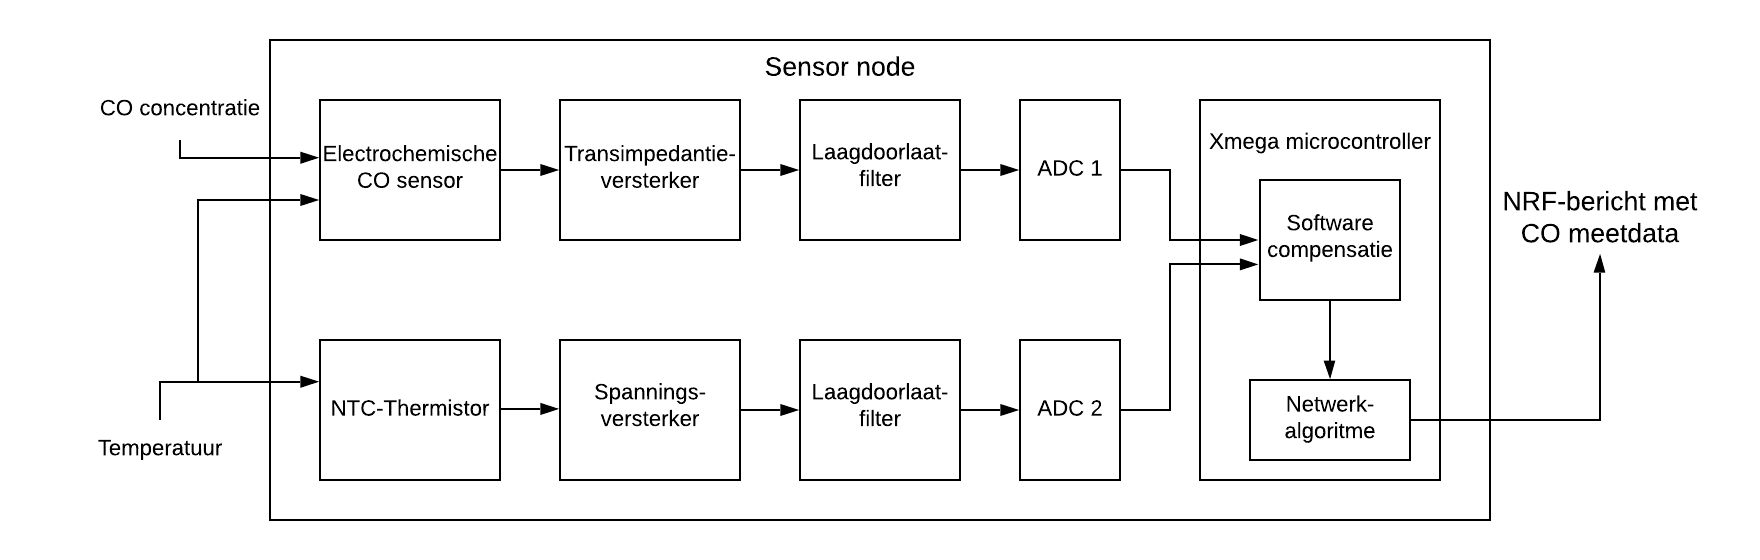
\includegraphics[width=1.7\linewidth]{../Media/sensorNode_dia.png}
		\caption{Blokdiagram van het complete systeem van de sensornode}
		\label{fig::sensorNode_dia}
	\end{figure}
	\newpage
	\section{Elektrochemische CO-sensor }
	In dit hoofdstuk wordt er besproken wat er nodig is om de elektrochemische CO-sensor te laten werken en wat de nodige signaalverwerking is om de sensor correct uit te kunnen lezen. Als elektrochemische CO-gassensor is er gekozen voor de \textit{3SP\_CO\_1000 package 110-102}
	%----------------------------------------------------------------------------------------
	\newpage
	
	\begin{thebibliography}{9}
		\bibliographystyle{IEEEtran}
		\bibitem{Effecten Koolmonoxide}
		Mariët Ticheler, 
		2008 [Bekeken in september 2019],
		[Rapport],
		"Koolmonoxide",
		Beschikbaar: \url{https://www.leefmilieu.nl/sites/www3.leefmilieu.nl/files/imported/pdf_s/MGM_2008-02_koolmonoxide.pdf}
		
		\bibitem{RIVM huurwoningen}
		M. van Bruggen, J.T.M. Gram, E.L. Boels, L. Ruhaak, M. Mooij,
		RIVM,
		2009 [Bekeken in september 2019],
		[Rapport],
		"Koolmonoxide in huurwoningen in de Randstad",
		Beschikbaar: \url{https://www.rivm.nl/bibliotheek/rapporten/609300009.pdf}
		
		\bibitem{Blootstelling aan CO}
		M. Mooij,
		RIVM,
		2008 [Bekeken in september 2019],
		[Rapport],
		"Chronische blootstelling aan koolmonoxide, tabel 2.2",
		Beschikbaar: \url{https://www.rivm.nl/bibliotheek/rapporten/609300005.pdf}
		
		\bibitem{NO2_Amsterdam}
		RIVM, J.p. Wesseling, S. van der Zee, P.L. Nguyen,
		2008 [Bekeken in september 2019],
		[Rapport],
		"Gemeten en berekende NO2-concentraties in Amsterdam in 2008",
		Beschikbaar: \url{https://www.rivm.nl/bibliotheek/rapporten/680705015.pdf}
		
		\bibitem{grafiek}
		Rijksinstituut voor Volksgezondheid
		2019[Bekeken in september 2019],
		[Online],
		"Meetgegevens NO2",
		Beschikbaar: \url{https://www.luchtmeetnet.nl}
		
		\bibitem{B4DF}
		Alphasense
		2018[Bekeken in september 2019],
		[Datasheet],
		"Datasheet",
		Beschikbaar: \url{http://www.alphasense.com/WEB1213/wp-content/uploads/2018/12/NO2B43F.pdf}
		
		\bibitem{xmega}
		978-90-484-3527-2,
		W. Dolman,
		2016[Bekeken in september 2019],
		[boek],
		"De taal C en de Xmega (2e druk)",
		Culemborg,
		Free Musketeers uitgeverij en productie
		
		\bibitem{SGX Intro}
		SGX Sensortech,
		01-02-2007 [Bekeken in oktober 2019],
		[Online],
		"Introduction to Electrochemical (EC) Gas Sensors",
		Beschikbaar: \url{https://www.sgxsensortech.com/content/uploads/2014/08/Introduction-to-Electrochemical-EC-Gas-Sensors1.pdf}
		
		\bibitem{MO sensoren}
		N. Barsan, U. Weimar,
		Institute of Physical and Theoretical Chemistry, University of Tuebingen,
		[Bekeken in september 2019],
		[Artikel],
		"Fundamentals of Metal Oxide Gas Sensors",
		Beschikbaar: \url{https://www.google.com/url?sa=t\&rct=j\&q=&esrc=s\&source=web\&cd=9\&ved=2ahUKEwjDwY__icTlAhVGJFAKHceND0gQFjAIegQIABAC\&url=https%3A%2F%2Fwww.ama-science.org%2Fproceedings%2FgetFile%2FBGx1&usg=AOvVaw0HkmkgTDH_rmiX19YCcaHD}
		
		\newpage
		\bibitem{Sensor keuze}
		H. Li, X. Mu, Y. Yang, A. J. Mason,
		IEEE,
		2014 [Bekeken in september 2019],
		[Artikel],
		"Low power Multi-mode Electrochemical Gas
		Sensor Array System for Wearable Health and
		Safety Monitoring",
		Beschikbaar: \url{https://ieeexplore.ieee.org/document/6851860}
		
		\bibitem{Thermistor}
		Ametherm Inc.
		2015 [Bekeken in november 2019],
		[Online],
		"NTC Thermistors – Temperature Measurement With A Wheatstone Bridge",
		Beschikbaar: \url{https://www.ametherm.com/thermistor/ntc-thermistors-temperature-measurement-with-wheatstone-bridge}
		
		\bibitem{SGX datasheet}
		SGX Sensortech,
		[Bekeken in oktober 2019],
		[Datasheet],
		"SGX-4CO Industrial Carbon Monoxide Sensor",
		Beschikbaar: \url{https://www.sgxsensortech.com/content/uploads/2014/07/DS-0138-SGX-4CO-V2.pdf}

		\bibitem{Hatech}
		HATECH gasdetectietechniek,
		[Bekeken in oktober 2019],
		[Online],
		"Onderhoud gasdetectoren",
		Beschikbaar: \url{https://www.hatechgas.com/onderhoud/geen-kalibratie-nodig/}	
		
	\end{thebibliography}
\end{document}
